\section{Articulated bodies\label{articulatedBodies}}

\subsection{Approaches to constraints\label{approachesToConstraints}}
The methods developed so far allow the simulation of a single rigid body with forces
acting on it. Further challenges arise when we consider multibody systems in which there are
conditions which must not be violated. In an articulated body, for example, each segment
must be modelled as an individual rigid body, under the condition that joints must not be pulled
apart.

There are various strategies for simulating articulated bodies:

\begin{itemize}
\item \emph{Penalty methods} conceptually join bodies together with springs so that when they
    begin to separate, a restoring force causes them to move back together again. These methods
    are simple to implement initially but hard to get right: if the springs are too weak, the
    bodies will separate too far; if they are too stiff, very large forces can arise suddenly,
    causing the simulation to become unstable.

\item Mechanics formulations using \emph{generalized coordinates}
    \cite{Hand:98,Goldstein:80,Featherstone:87,Wilhelms:91} build constraints firmly into
    the system: the number of generalized coordinates equals the actual number of degrees of
    freedom after the constraints have been applied. The state of the system is specified only in
    terms of these generalized coordinates, and they are chosen such that the system will always
    be in a legal state, irrespective of what the values of the coordinates are. These algorithms
    allow efficient and reliable computation. However, the equations are only tractable for
    so-called \emph{holonomic constraints} (definition in~\cite{Hand:98}), which excludes
    many interesting systems.

\item This project makes a compromise between the flexibility of penalty methods and the stability
    of generalized coordinates. As in the penalty method, we initially treat each segment of an
    articulated body separately. The constraints are then formulated in such a way that we can
    not only tell whether the system is currently in an illegal state, but also whether it is
    moving towards one, and even whether it is accelerating towards one. Using the method of
    \emph{Lagrange multipliers} we can determine what forces must be applied to the bodies to
    nullify this unwanted acceleration before it ever occurs. This compromise comes at the
    expense of higher computational cost, because simultaneous linear equations have to be solved
    at run-time.
\end{itemize}

The mathematical formulation of Lagrange multipliers is derived in~\cite{BaraffWitkin:97} and
extended in~\cite{Saunders:PhD} (also see~\cite{Baraff:96} for an optimized algorithm),
and I only state the results here.


\subsection{Lagrange multipliers\label{lagrange}}

Each constraint effectively reduces the number of degrees of freedom by one, and is expressed
as a function $c$ which is zero when the constraint is satisfied. (A ball-and-socket
joint, which allows three modes of rotation but no separation, reduces the number of d.o.f.\ by
three and is therefore expressed as a vector of three scalar constraint functions.) All constraint
functions can then be concatenated into a single constraint vector \ve{c}.

The constraints can be satisfied by solving the equation\footnote{Here the sign convention
of~\cite{BaraffWitkin:97} is adopted, which is the opposite of~\cite{Saunders:PhD}.}
\begin{equation}
\label{lagrangeEquation}
-\m{J}\m{M}^{-1}\m{J}^T\ve{\lambda} = \dot{\m{J}}\dot{\ve{x}} +
    \m{J}\m{M}^{-1}(\ve{\Phi} + \ve{\Phi}_p) + k\ve{c} + d\dot{\ve{c}}.
\end{equation}
The values of all variables except for the vector $\ve{\lambda}$ in this equation are
known, and they are explained in appendix~\ref{constraintPrerequisites}. In brief, they are:

\vspace{10pt}
\begin{tabular}{@{}ll}
\ve{c}, $\dot{\ve{c}}$ & Constraint vector and its first derivative w.r.t.\ time.\\
\m{J}, $\dot{\m{J}}$ & Jacobian matrices derived from \ve{c} (see appendix~\ref{jacCalculation}).\\
\m{M} & Mass-inertia matrix combining the masses and moments of inertia\\
      & of all bodies in the scene. \\
$\dot{\ve{x}}$ & Combined linear and angular velocity vector of all bodies.\\
\ve{\Phi} & Combined forces and torque vectors acting on all bodies.\\
$\ve{\Phi}_p$ & Effects of free precession.\\
$k$, $d$ & Scalar constants regulating error compensation, discussed
    in~\cite{BaraffWitkin:97}.
\end{tabular}
\vspace{10pt}

For us it will suffice to consider this equation to be a `black box' which can be
given to a linear equation solver to obtain $\ve{\lambda}$.

$\ve{\lambda}$ is an $m$-row vector of so-called \emph{Lagrange multipliers} (after which this
algorithm is named), where $m$ is the number of constraints. Once we have solved for it, we can
compute the expression
\begin{equation} \label{lagrangeSolution}
\ve{\Phi}_c = \m{J}^T\,\ve{\lambda}.
\end{equation}
$\ve{\Phi}_c$ is the vector of constraint restoring forces and torques for all bodies.
Speaking in physical terms, these are the reaction forces which balance the action \ve{\Phi}.
All we therefore need to do is to compute $\ve{\Phi} + \ve{\Phi}_c$ and to feed the result into
our ODE solver, and the motion which ensues will satisfy the constraints.
$\ve{\Phi}_p$ must not be added to this term\footnote{provided the moments of inertia are
recalculated based on the bodies' orientation at every time step.}.


\subsection{Modelling the human body}

The human body's selection of joint types is quite limited compared to the range of connectors
found in machines~\cite{Kalra:95}: for example, there are no sliding joints or screws. The simple
types of joint found in human bodies are ball-and-socket joints allowing rotation about three axes
(like shoulders and hips), and revolute joints limited to a single axis (like knees and elbows).
The issue is made more complicated by compound joints like the spine, and motion which occurs
along the length of a segment rather than at a joint (like rotating the wrist about the axis of
the lower arm, which occurs through a relative shift of the ulna and radius
bones~\cite{Anatomy:03}).

To make the model manageable, I chose to be anatomically ignorant and assumed that two adjacent
segments of an articulated body are connected by a single joint, and that rotation occurs only
about this joint. Each bone has a local coordinate system whose origin lies at the joint to the
parent bone. This is illustrated in figure~\ref{jointsFigure}.

\begin{figure}
\centerline{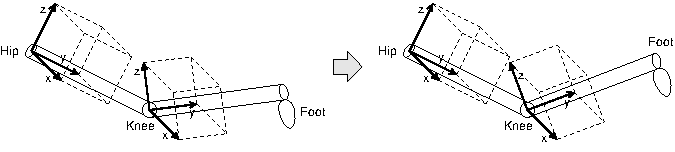
\includegraphics{figures/joint1}}
\caption{Two bones connected by a revolute joint, e.g.\ a knee. Rotation is constrained to be
    possible only about the local x~axis of the knee, but not the local y~axis
    (the lower leg itself) or the local z~axis (sideways).\label{jointsFigure}}
\end{figure}

There are different ways of formulating this model. My approach is to assume initially that every
joint is a ball-and-socket type. For those joints which are not, additional constraints are
added to restrict the permitted axes of rotation.

\subsection{Ball-and-socket joints}

The position of a joint is a particular offset from the centre of mass in one body's frame, and a
different offset from the other body's centre of mass. While the bodies may move around, these
offsets stay constant (as seen in the body's frame).

Figure~\ref{ballAndSocketFigure} gives an example: here, the configuration of bodies satisfies the
ball-and-socket constraint iff $\ve{a}+\ve{s} = \ve{b}+\ve{t}$, i.e.\ if the joint has not
separated. We can rewrite this to give the constraint function
\begin{equation}
\ve{c} = \ve{a} + \ve{s} - \ve{b} - \ve{t}
\end{equation}
which equals \ve{0}, the three-dimensional null vector, iff the constraint is satisfied.

\begin{figure}
\psfrag{frag:o}{\ve{O}}
\psfrag{frag:a}{\ve{a}}
\psfrag{frag:b}{\ve{b}}
\psfrag{frag:s}{\ve{s}}
\psfrag{frag:t}{\ve{t}}
\centerline{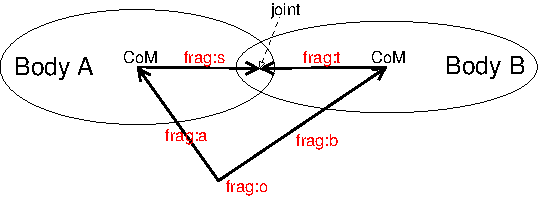
\includegraphics{figures/joint2}}
\caption[]{A valid ball-and-socket joint configuration. \ve{s} is constant in body~A's frame,
    while \ve{t} is constant in the frame of body~B. In the world frame, these two vectors
    therefore rotate according to their respective body's orientation.\label{ballAndSocketFigure}}
\end{figure}

\subsection{Rotation constraints\label{rotationConstraints}}

In the case of an elbow or a knee, we also need to prohibit the rotation about particular axes.
After some thought I came up with the constraint function
\begin{equation}\label{rotationConstraintEqn}
c = \Re(\tilde{\ve{n}}\q{p}^{-1}\q{q})
\end{equation}
in which \q{p} is the quaternion of orientation for body~A, \q{q} the quaternion for body~B, and
\ve{n} a vector pointing along the prohibited axis in body~A's frame. Setting $c$ to zero ensures
that no rotation occurs about the axis~\ve{n}. If two different axes are prohibited with two
separate constraints, then rotation is only possible about a single axis orthogonal to the two
prohibited axes. Further details on this constraint are given in appendix~\ref{constrJoystick}.

\subsection{Angle limitation\label{angleLimitation}}

The constraints described so far capture most of the features of the human skeleton, with one
exception: if rotation is permitted about some axis, there is no limit to the amount of rotation
that can occur. For example, permitting a human to look left and right would allow the simulation
to rotate his head by an arbitrary amount. Imposing
limits on the angle of rotation as well as the axis is possible but more complicated, and will
be explained in section~\ref{generalizedCollisions}. It is worth noting that this is our
first example of a non-holonomic constraint, and thus lies beyond the capabilities of
generalized-coordinate approaches.
